\documentclass[GBK,winfonts,a4paper,10pt]{ctexart}
\usepackage{fancyhdr}
\usepackage{indentfirst}
\usepackage{graphics}
\usepackage{enumerate}
\usepackage{framed}
\usepackage{amsmath}
\usepackage{graphicx}
\usepackage{setspace}
\usepackage{hyperref}
\usepackage{mdwlist}
\usepackage{algorithm}
\usepackage{algorithmic}
\usepackage{listings}
\usepackage{xcolor}
\usepackage{marvosym,listings,etoolbox}
\usepackage{geometry}

\lstset{numbers=left, numberstyle=\small, keywordstyle=\color{blue!70}, commentstyle=\color{red!50!green!50!blue!50}, frame=shadowbox, rulesepcolor=\color{red!20!green!20!blue!20},escapeinside=``, xleftmargin=2em,xrightmargin=2em, aboveskip=1em, literate={@}{\MVAt}1}

\patchcmd{\verb}{\dospecials}{\dospecials\atspecial}{}{}
\def\atspecial{\begingroup\lccode`~=`@
  \lowercase{\endgroup\let~}\MVAt
  \catcode`@=\active}
  


\newcommand{\tabincell}[2]{\begin{tabular}{@{}#1@{}}#2\end{tabular}}%
       
\lstdefinestyle{customc}{
  belowcaptionskip=1\baselineskip,
  breaklines=true,
  frame=single,
  xleftmargin=\parindent,
  language=C,
  showstringspaces=false,
  basicstyle=\fontsize{8pt}{8pt}\ttfamily,
  keywordstyle=\bfseries\color{green!40!black},
  commentstyle=\itshape\color{purple!40!black},
  identifierstyle=\color{blue},
  stringstyle=\color{orange},
  tabsize=4,
  numbers=none,
  mathescape=false,
}

\lstset{escapechar=@,style=customc}

\pagestyle{fancy}
\hypersetup{pdfborder=0 0 0}

\usepackage{clrscode}

\usepackage{latexsym}

\begin{document}

\rhead{}
\lhead{}
\cfoot{\thepage}
\renewcommand{\footrulewidth}{0.4pt}
%\renewcommand{\thesection}{}
\renewcommand{\algorithmicrequire}{\textbf{Input:}}
\renewcommand{\algorithmicensure}{\textbf{Output:}}
\setlength{\tabcolsep}{2pt}

\setlength{\parindent}{2em}

\thispagestyle{fancy}


\title{Operating System MIT 6.828 JOS Lab4 Report}
\author{Computer Science \\ ChenHao(1100012776) }
\date{\today}
\maketitle

\thispagestyle{fancy}

\tableofcontents

\newpage

\begin{section}{Part A: Multiprocessor Support and Cooperative Multitasking}
\begin{subsection}{Exercise 1}
\par
这是是要我们实现一个用于简单分配内存空间进行映射的函数,利用以前写的boot\_map\_region就可以很容易的实现。
\begin{lstlisting}[language=C]
void *
mmio_map_region(physaddr_t pa, size_t size)
{
	static uintptr_t base = MMIOBASE;

	pa = ROUNDDOWN(pa, PGSIZE);
	boot_map_region(kern_pgdir, base, ROUNDUP(size, PGSIZE), pa, PTE_PCD | PTE_PWT | PTE_W);
	uintptr_t tmp_base = base;
	base += ROUNDUP(size, PGSIZE);
	return (void *) tmp_base;
}
\end{lstlisting}
\end{subsection}

\begin{subsection}{Exercise 2}
\par
这一段是在说明AP是如何启动的,BSP在启动APs前,会先收集CPU信息,APIC IDs, LAPIC的MMIO地址等信息,然后执行boot\_aps,在这段中BSP依次让每个AP启动执行mpentry.S中的代码(BSP将代码复制至内存中MPENTRY\_ADDRESS的位置,并将每个的AP的CS:IP设置好),通过发送STARTUP IPI两次来启动AP(在lapic\_startup函数中说明了,这个启动方式是硬件支持的)之后AP就执行启动程序,等执行完后会给BSP发送CPU\_STARTED的信号。表示结束,BSP在APs的启动过程中一直处于空循环的状态。
\par
因此MPENTRY\_ADDRESS所在的内存地址是不能够被用于分配其它代码或者数据的,因此在page\_init的需要进行修改。
\begin{lstlisting}[language=C]
void
page_init(void)
{
    page_free_list = NULL;
    size_t i;
	size_t nf_lb = IOPHYSMEM / PGSIZE;
    size_t nf_ub = PADDR(boot_alloc(0)) / PGSIZE;
    size_t mpentry_page = MPENTRY_PADDR / PGSIZE;
    for (i = 0; i < npages; i++) {
        if (i != 0 && (i < nf_lb || i >= nf_ub) && i != mpentry_page) {
		    pages[i].pp_ref = 0;
            pages[i].pp_link = page_free_list;
		    page_free_list = &pages[i];
        } else {
            pages[i].pp_ref = 1;
            pages[i].pp_link = NULL;
        }
	}
}
\end{lstlisting}
\end{subsection}

\begin{subsection}{Question 1}
\par
kern/mpentry.S的链接地址在KERNBASE以上,而AP在是在实模式下无法使用页寻址,因此我们需要手动地计算出其所在的物理地址。如果注释了这句,则会产生缺页异常。
\end{subsection}

\begin{subsection}{Exercise 3}
\par
问题:为什么给kern\_pgdir即可,不用每个cpu的pgdir都赋予值?
\par
因为每个cpu的pgdir在高位都是相同的,即内核部分除了内核栈不同外,代码和数据都是映射到相同的地址下。
\begin{lstlisting}[language=C]
static void
mem_init_mp(void)
{    
    int cpu_id;
    for (cpu_id = 0; cpu_id < NCPU; cpu_id++) {
        boot_map_region(kern_pgdir,
                        KSTACKTOP - cpu_id * (KSTKSIZE + KSTKGAP) - KSTKSIZE,
                        KSTKSIZE,
                        PADDR(percpu_kstacks[cpu_id]),
                        PTE_W);
    }
}
\end{lstlisting}
\end{subsection}

\begin{subsection}{Exercise 4}
\par
根据cpu\_id放置在对应的位置即可。
\begin{lstlisting}[language=C]
void
trap_init_percpu(void)
{
	// LAB 4: Your code here:
    int cpu_id = thiscpu->cpu_id;
    thiscpu->cpu_ts.ts_esp0 = KSTACKTOP - cpu_id * (KSTKSIZE + KSTKGAP);
    thiscpu->cpu_ts.ts_ss0 = GD_KD;

    gdt[(GD_TSS0 >> 3) + cpu_id] = SEG16(STS_T32A, (uint32_t) (&(thiscpu->cpu_ts)),
    							sizeof(struct Taskstate), 0);
    gdt[(GD_TSS0 >> 3) + cpu_id].sd_s = 0;

    ltr(GD_TSS0 + (cpu_id << 3));

    lidt(&idt_pd);
}
\end{lstlisting}
\end{subsection}

\begin{subsection}{Exercise 5}
\par
根据题目要求在对应的地方放上lock或者unlock即可,连位置都有注释提示,非常简单。
\end{subsection}

\begin{subsection}{Question 2}
\par
共享内核栈是会存在问题的,在发生中断的时候,对于现场保护的是发生在big kernel lock之前的,因此当共享内核栈很可能会产生参数的混乱。
\end{subsection}

\begin{subsection}{Exercise 6}
\par
这一部分要我们实现Round-Robin Scheduling,即类似循环链表,每次从刚执行的env之后选择最近的一个RUNNABLE的进行执行。代码如下:
\begin{lstlisting}[language=C]
void
sched_yield(void)
{
	struct Env *idle;

	// LAB 4: Your code here.
	int now_env, i;
	if (curenv) {			// thiscpu->cpu_env
		now_env = (ENVX(curenv->env_id) + 1) % NENV;
	} else {
		now_env = 0;
	}
	for (i = 0; i < NENV; i++, now_env = (now_env + 1) % NENV) {
		if (envs[now_env].env_status == ENV_RUNNABLE) {
			//cprintf("I am CPU %d , I am in sched yield, I find ENV %d\n", thiscpu->cpu_id, now_env);
			env_run(&envs[now_env]);
		}
	}
	if (curenv && curenv->env_status == ENV_RUNNING) {
		env_run(curenv);
	}
	// sched_halt never returns
	sched_halt();
}
\end{lstlisting}
\end{subsection}

\begin{subsection}{Question 3-4}
\par
Question 3: 由于Env在mem\_init中分配了内存进行存储并建立了映射,而这个映射在每个CPU上都是一致的,因此lcr3()后对于Env的还是存在虚拟内存到物理内存的映射的。
\par
Question 4: 保存现场是为了之后CPU进行继续处理这个environment的时候保证不会造成错误。保护现场发生在发生中断的情况下,这时候堆栈上储存了当前environment的信息,之后再通过curenv->env\_tf = *tf来保存在environment中。
\end{subsection}

\begin{subsection}{Challenge 2}
\par
设置一个带有优先级的调度,我实现了一个非常弱智的,每次找到可运行的优先级最高的,如果优先级相同,则优先处理刚处理完的进程号之后最近的一个进程。对于优先级的表示,我在struct Env中设置了一位env\_priority表示优先级,越大表示优先级越高。
\par
因此调度就变为了:
\begin{lstlisting}[language=C]
void
sched_yield(void)
{
	struct Env *idle;

	int now_env, i;
	if (curenv) {			// thiscpu->cpu_env
		now_env = (ENVX(curenv->env_id) + 1) % NENV;
	} else {
		now_env = 0;
	}
	uint32_t max_priority = 0;
	int select_env = -1;
	for (i = 0; i < NENV; i++, now_env = (now_env + 1) % NENV) {
		if (envs[now_env].env_status == ENV_RUNNABLE && (envs[now_env].env_priority > max_priority || select_env == -1)) {
			//cprintf("I am CPU %d , I am in sched yield, I find ENV %d\n", thiscpu->cpu_id, now_env);
			select_env = now_env;
			max_priority = envs[now_env].env_priority;
		}
	}
	if (select_env >= 0 && (!curenv || curenv->env_status != ENV_RUNNING || max_priority >= curenv->env_priority)) {
		env_run(&envs[select_env]);
	}
	
	if (curenv && curenv->env_status == ENV_RUNNING) {
		env_run(curenv);
	}

	// sched_halt never returns
	sched_halt();
}
\end{lstlisting}
\par
为了测试,我首先增加了一个更改priority的系统调用:
\begin{lstlisting}[language=C]
static int
sys_set_priority(envid_t envid, uint32_t new_priority)
{
	struct Env * env;
	int r = envid2env(envid, &env, 1);	
	if (r < 0) return -E_BAD_ENV;
	
	env->env_priority = new_priority;
	return 0;
}
\end{lstlisting}
\par
我在用户fork()库函数增加了一个static变量num,使得其递减,并设置刚创建的子进程的priority为num:
\begin{lstlisting}[language=C]
envid_t
fork(void)
{
	static int num = 0x100;

	// LAB 4: Your code here.
	set_pgfault_handler(pgfault);
	int childpid = sys_exofork();
	if (childpid < 0) {
		panic("fork sys_exofork error : %e\n", childpid);
	}
	int r;

	if (childpid == 0) {
		......
	} else {
		......

		// LAB 4 Challenge , set childenv's priority
		num--;
		if (num == 0) num = 0x100;
		r = sys_set_priority(childpid, num);
		if (r < 0) panic("fork, set priority error\n");

		// mark the child as runnable and return
		r = sys_env_set_status(childpid, ENV_RUNNABLE);
		if (r < 0) panic("fork, set child process to ENV_RUNNABLE error : %e\n", r);
		return childpid;
	}
}
\end{lstlisting}
\par
这样就可以进行测试了,我把hello.c更改为了下面的代码,根据我们之前的铺垫,预期就是执行完子进程0,才会执行子进程1,才会执行子进程2,才会执行子进程3.
\begin{lstlisting}[language=C]
#include <inc/lib.h>

void
umain(int argc, char **argv)
{
	cprintf("hello, world\n");
	cprintf("i am environment %08x\n", thisenv->env_id);

	int i, child, j;
	for (i = 0; i != 3; i++) {
		child = fork();
		if (child == 0) {
			for (j = 0; j != 10; j++) {
				cprintf("hello world from : %d\n", i);
				sys_yield();
			}
			break;
		}
	}
}
\end{lstlisting}
\par
和预期一致!
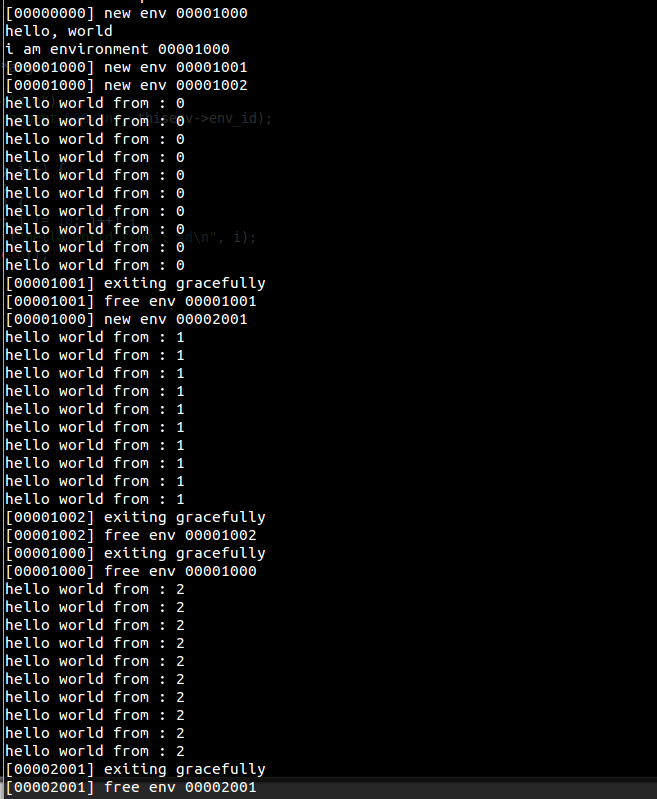
\includegraphics[scale=0.5]{ch2.png}
\end{subsection}

\begin{subsection}{Question 7}
\begin{subsubsection}{sys\_exofork}
\par
这个部分是生成一个新的environment,使得其寄存器的值与当前的environment的一样,对于新的environment返回值为0(\%eax=0)。对于该函数返回新的environment的pid号。
\begin{lstlisting}[language=C]
static envid_t
sys_exofork(void)
{
	struct Env * new_env;
	int r = env_alloc(&new_env, curenv->env_id);
	if (r < 0) return r;
	
	new_env->env_status = ENV_NOT_RUNNABLE;
	memcpy((void *)(&new_env->env_tf), (void*)(&curenv->env_tf), sizeof(struct Trapframe));
	
	// for children environment, return 0
	new_env->env_tf.tf_regs.reg_eax = 0;

	return new_env->env_id;
}
\end{lstlisting}
\end{subsubsection}

\begin{subsubsection}{sys\_env\_set\_status}
\par
这个是设置environment的status,按照注释做即可。
\begin{lstlisting}[language=C]
static int
sys_env_set_status(envid_t envid, int status)
{
	if (status != ENV_RUNNABLE && status != ENV_NOT_RUNNABLE) 
		return -E_INVAL;

	struct Env * env;
	int r = envid2env(envid, &env, 1);
	if (r < 0) return r;
	env->env_status = status;
	return 0;
}
\end{lstlisting}
\end{subsubsection}

\begin{subsubsection}{sys\_page\_alloc}
\par
这个函数是为environment创建虚拟地址va的映射页,按照注释一条一条做即可。注意如何无法建立映射,则新分配的页需要释放掉。
\begin{lstlisting}[language=C]
static int
sys_page_alloc(envid_t envid, void *va, int perm)
{
	struct Env * env;
	int r = envid2env(envid, &env, 1);
	if (r < 0) return -E_BAD_ENV;

	if ((uint32_t)va >= UTOP || ROUNDUP(va, PGSIZE) != va) return -E_INVAL;
	
	if (!((perm & PTE_U) && (perm & PTE_P) && (perm & (~PTE_SYSCALL))==0)) return -E_INVAL;

	struct PageInfo * pg = page_alloc(ALLOC_ZERO);
	if (pg == NULL) return -E_NO_MEM;
	if (page_insert(env->env_pgdir, pg, va, perm) < 0) {
		// page_insert fails, should free the page you allocated!  
		page_free(pg);
		return -E_NO_MEM;
	}
	return 0;
}
\end{lstlisting}
\end{subsubsection}

\begin{subsubsection}{sys\_page\_map}
\par
按照给定的进程,和虚拟地址,拷贝其映射至另一个进程的给定的虚拟地址上,按照注释一条一条做即可。
\begin{lstlisting}[language=C]
static int
sys_page_map(envid_t srcenvid, void *srcva,
	     envid_t dstenvid, void *dstva, int perm)
{
	struct Env * dstenv, * srcenv;
	int r = envid2env(dstenvid, &dstenv, 1);
	if (r < 0) return -E_BAD_ENV;
	r = envid2env(srcenvid, &srcenv, 1);
	if (r < 0) return -E_BAD_ENV;

	if ((uint32_t)srcva >= UTOP || ROUNDUP(srcva, PGSIZE) != srcva) return -E_INVAL;
	if ((uint32_t)dstva >= UTOP || ROUNDUP(dstva, PGSIZE) != dstva) return -E_INVAL;


	// struct PageInfo * page_lookup(pde_t *pgdir, void *va, pte_t **pte_store)
	struct PageInfo * pg;
	pte_t * pte;
	pg = page_lookup(srcenv->env_pgdir, srcva, &pte);
	if (pg == NULL) return -E_INVAL;		

	if (!((perm & PTE_U) && (perm & PTE_P) && (perm & (~PTE_SYSCALL))==0)) return -E_INVAL;
	
	if ((perm & PTE_W) && ((*pte) & PTE_W) == 0) return -E_INVAL;

	// int page_insert(pde_t *pgdir, struct PageInfo *pp, void *va, int perm)
	if (page_insert(dstenv->env_pgdir, pg, dstva, perm) < 0) return -E_NO_MEM;

	return 0;
}
\end{lstlisting}
\end{subsubsection}

\begin{subsubsection}{sys\_page\_unmap}
\par
按照注释一条一条做即可。
\begin{lstlisting}[language=C]
static int
sys_page_unmap(envid_t envid, void *va)
{
	struct Env * env;
	int r = envid2env(envid, &env, 1);
	if (r < 0) return -E_BAD_ENV;

	if ((uint32_t)va >= UTOP || ROUNDUP(va, PGSIZE) != va) return -E_INVAL;
	
	// void page_remove(pde_t *pgdir, void *va)
	page_remove(env->env_pgdir, va);

	return 0;
}
\end{lstlisting}	
\end{subsubsection}

\par
注意到目前写的调度都是执行完一个environment之后就结束,剩余最后一个作为monitor,其余的CPU均HLT住,但是注意不能把所有CPU都HLT,这样会出现中断13。当我尝试在init.c中设置environment的数量大于CPU核的数量的时候,就会造成中断13,因为所有的CPU都HLT了。我在这里调试了很久,花了很长时间,最后才发现竟然是没考虑清楚。
\end{subsection}

\end{section}

\begin{section}{Part B: Copy-on-Write Fork}
\par
fork()指令会根据当前进程生成一个新的与原进程一样的(除了pid号不一样)的进程,他们拥有独立的内存空间,独立的寄存器,独立的用户栈等等。因此我们对于fork()的执行需要将内存中完全复制一份,这个代价是非常高的。我们可以采用Copy-on-Write的技术,使用Copy-on-Write的原因在于,fork()中有的内存是多个进程是只读的,那么我们完全可以将这部分的内存不进行复制;其次并不是所有的数据都需要更改,所以我们可以共同使用同一个物理内存,当进行写操作的时候,再分为独立的内存。其次还有一个原因是许多情况下fork()之后会执行exec(),因此fork()采用Copy-on-Write是一个比较很好的减少不必要操作,节省内存的一个方法。
\par
如何得知某一块内存是被多个进程共用,如何得知这样的内存在被写的时候需要进行复制。对于前一个问题,PTE表项中有由一个专门的标志为PTE\_COW,表示这个页是否使用了Copy-on-Write。如何在写的时候进行复制,这里采用触发Page Fault的方法。JOS在内核中注册了一个Page fault的处理程序,允许用户进程将自己的页错误函数注册到进程结构中。这样当发生页错误的时候可以在user-level下实现对page level的处理,增大了灵活性,而且一定程度下节省了page fault霸占内核的时间。
\par
为了实现user-level的page fault,那么就不能使用内核栈用于保存信息,因此就出现了Exception Stack,是user-level page fault handler运行时用的栈,用于保存信息。

\begin{subsection}{Exercise 8}
\par
如果用户需要使用自己的Page Fault Handler,则事先需要向内核注册handler所在的位置,保存在用户进程的env\_pagfalut\_upcall变量中,此处就是注册user-level page fault handler。
\begin{lstlisting}[language=C]
static int
sys_env_set_pgfault_upcall(envid_t envid, void *func)
{
	struct Env * env;
	int r = envid2env(envid, &env, 1);
	if (r < 0) return r;

	env->env_pgfault_upcall = func;
	return 0;
}
\end{lstlisting}
\end{subsection}

\par
当产生Page Fault的时候,如果是内核模式下产生的,则产生panic,一定是系统出现了bug。如果是用户模式下产生的page fault且存在user-level page fault的handler的时候,则需要保存现场信息至user exception stack。并设置好当前env的eip为user-level page fault handler的入口地址,并将栈指向当前user exception stack的位置。然后返回用户态执行user-level page fault handler。特别要注意在user-level page fault handler中,是在用户模式下执行的,并且所使用的栈是在user exception stack上。当user-level page fault handler执行完成后,会切换会用户进程和用户运行栈下继续执行。
\begin{subsection}{Exercise 9}
\par
此处就为kernel在接受到page\_fault异常的时候,进行的处理。如果是在用户模式且存在注册的page fault handler,则需要存栈。如果是page fault嵌套,则需要在异常栈开始的地方多压一个空的32-bit word。为什么要这样做,后面的exercise会进行解释。
\begin{lstlisting}[language=C]
void
page_fault_handler(struct Trapframe *tf)
{
	uint32_t fault_va;

	// Read processor's CR2 register to find the faulting address
	fault_va = rcr2();

	// Handle kernel-mode page faults.

	// LAB 3: Your code here.
	if (tf->tf_cs == GD_KT)
    	panic("page_fault_handler : page fault in kernel\n");
    
    	if (curenv->env_pgfault_upcall != NULL) {
    		// exist env's page fault upcall
		
   	 	struct UTrapframe * ut;
   	 	if (tf->tf_esp >= UXSTACKTOP - PGSIZE && tf->tf_esp <= UXSTACKTOP - 1) {
    			// already in user exception stack, should first push an empty 32-bit word
    			ut = (struct UTrapframe *)((void *)tf->tf_esp - sizeof(struct UTrapframe) - 4);
	 	   	user_mem_assert(curenv, (void *)ut, sizeof(struct UTrapframe) + 4, PTE_U | PTE_W);
  	  	} else {
    			// it's the first time in user exception stack
    			ut = (struct UTrapframe *)(UXSTACKTOP - sizeof(struct UTrapframe));
		    	user_mem_assert(curenv, (void *)ut, sizeof(struct UTrapframe), PTE_U | PTE_W);
   	 	}
    	
    		ut->utf_esp = tf->tf_esp;
   	 	ut->utf_eflags = tf->tf_eflags;
   	 	ut->utf_eip = tf->tf_eip;
		ut->utf_regs = tf->tf_regs;
		ut->utf_err = tf->tf_err;
		ut->utf_fault_va = fault_va;

		curenv->env_tf.tf_eip = (uint32_t)curenv->env_pgfault_upcall;
		curenv->env_tf.tf_esp = (uint32_t)ut;
   	 	env_run(curenv);
    } 

	// Destroy the environment that caused the fault.
	cprintf("[%08x] user fault va %08x ip %08x\n",
		curenv->env_id, fault_va, tf->tf_eip);
	print_trapframe(tf);
	env_destroy(curenv);
}
\end{lstlisting}
\end{subsection}

\begin{subsection}{Exercise 10}
\par
\_pgfault\_upcall实际上实现到真正handler的跳转,待handler处理完后进行环境的恢复。对于栈的恢复是比较简单的,因为old-esp和old-ebp已经存在了栈中,而对于eip的恢复就需要使用ret的机制,即弹出栈顶元素作为eip,跳转到eip的位置。因此我们在ret的之前只需要把eip存放在栈顶的位置即可,应该放在哪里?还记得如果产生了page fault的嵌套,则在栈中会多存放一个空的4字节,这就是用于返回eip的存放。对于第一层的page fault,则可以把eip放在原来的用户运行栈的下一个4字节位置,并将\%esp指向eip的位置,使用ret就可以实现跳转了。
\par
对于4字节是否是必须的?为什么不能在最后再将返回的\%eip弹入栈中?这是因为你是无法不污染寄存器的情况下实现这样的操作的,即为了在最后将\%eip弹入栈中,你必须需要寄存器来存储。而这样对于保存其值的寄存器便无法不被污染。
\begin{lstlisting}[language=C]
	// fix old esp
	movl 0x30(%esp), %eax
	subl $0x4, %eax
	movl %eax, 0x30(%esp)

	// set trap-time %eip
	movl 0x28(%esp), %ebx
	movl %ebx, (%eax)

	// Restore the trap-time registers.  After you do this, you
	// can no longer modify any general-purpose registers.
	addl $0x08, %esp 	// ignore err_code and fault_va
	popal 				// restore registers

	// Restore eflags from the stack.  After you do this, you can
	// no longer use arithmetic operations or anything else that
	// modifies eflags.
	addl $0x04, %esp 	// ignore eip 
	popfl				// modify eflags

	// Switch back to the adjusted trap-time stack.
	popl %esp

	// Return to re-execute the instruction that faulted.
	ret
\end{lstlisting}
\end{subsection}

\begin{subsection}{Exercise 11}
\par
这里实际上是提供给用户的库函数,需要做的有申请分配exception stack的空间,以及系统调用设置user-level page fault函数。注意给系统的实际上是\_pgfault\_upcall,这是user-level page fault的入口程序,在实际的handler存放在\_pgfault\_handler中,这样从内核态到用户态page fault的转换,实际上是到了\_pgfault\_upcall,再在其中实现到真正handler:\_pgfault\_handler的跳转。
\begin{lstlisting}[language=C]
void
set_pgfault_handler(void (*handler)(struct UTrapframe *utf))
{
	int r;
	if (_pgfault_handler == 0) {
		// First time through!	
		// LAB 4: Your code here.
		//int sys_page_alloc(envid_t envid, void *va, int perm)
		r = sys_page_alloc(0, (void*)(UXSTACKTOP - PGSIZE), PTE_U | PTE_W | PTE_P);
		if (r < 0) {
			panic("sys_page_alloc error : %e\n", r);
		}
		// how to know envid, put 0, envid2env will help us to get curenv in syscall
		r = sys_env_set_pgfault_upcall(0, _pgfault_upcall);		
		if (r < 0) {
			panic("sys_env_set_pgfault_upcall error : %e\n", r);
		}
	}
	// Save handler pointer for assembly to call.
	_pgfault_handler = handler;
}
\end{lstlisting}
\end{subsection}

\begin{subsection}{ Exercise 12 }
\par
这个部分就是要真正实现一个带Copy-on-Write的提供给用户的fork函数了。为了实现Copy-on-Write需要先注册一个pgfault\_handler,这样当某一个进程对某一块共享区域进行写入的时候,就绪要进行内存的复制使得这块内存不共享。然后进行sys\_exofork(),由于此时子进程还处于NOT\_RUNNABLE的状态,父进程需要对子进程构建内存的映射(这里只需要复制0~UTOP中存在的并且是用户的内存条目,对于内核态的数据和代码都是共享的,已经存在于子进程的页表中,无需拷贝),以及创建分配一块exception stack的内存,并设置子进程的pgfault\_handler。当这些都完成了,说明子进程已经可以开始运行了,就可以标记子进程的状态为RUNNABLE了。
\par
特别注意当子进程进行执行的时候,需要更新子进程的thisenv号。
\begin{subsubsection}{ fork }
\begin{lstlisting}[language = C]
envid_t
fork(void)
{
	set_pgfault_handler(pgfault);
	int childpid = sys_exofork();
	if (childpid < 0) {
		panic("fork sys_exofork error : %e\n", childpid);
	}
	int r;

	if (childpid == 0) {
		// child process
		// Remember to fix "thisenv" in the child process. ??? 
		thisenv = &envs[ENVX(sys_getenvid())];
		// cprintf("fork child ok\n");
		return 0;
	} else {
		// map page to new environment
		// kernel page is already in new environment
		uint32_t i;
		for (i = 0; i != UTOP; i += PGSIZE) 
		if ((uvpd[PDX(i)] & PTE_P) && (uvpt[i / PGSIZE] & PTE_P) && (uvpt[i / PGSIZE] & PTE_U)) {
			duppage(childpid, i / PGSIZE);
		}

		// allocate exception stack
		r = sys_page_alloc(childpid, (void *)(UXSTACKTOP - PGSIZE), PTE_U | PTE_W | PTE_P);
		if (r < 0) panic("fork, sys_page_alloc user exception stack error : %e\n", r);

		// set user environment user page fault handler 
		extern void _pgfault_upcall(void);
		r = sys_env_set_pgfault_upcall(childpid, _pgfault_upcall);
		if (r < 0) panic("fork, set pgfault upcall fail : %e\n", r);

		// mark the child as runnable and return
		r = sys_env_set_status(childpid, ENV_RUNNABLE);
		if (r < 0) panic("fork, set child process to ENV_RUNNABLE error : %e\n", r);

		// cprintf("fork father ok!");
		return childpid;
	}

	panic("fork not implemented");
}
\end{lstlisting}
\end{subsubsection}

\begin{subsubsection}{ duppage }
\par
这部分就是实现页表的复制,需要区分读和写即可。如果是读,则需要更改子进程的同时自己页表的标志位也需要更改。
\begin{lstlisting}[language = C]
static int
duppage(envid_t envid, unsigned pn)
{
	// do not dup exception stack
	if (pn * PGSIZE == UXSTACKTOP - PGSIZE) return 0;

	int r;
	void * addr = (void *)(pn * PGSIZE);
	if ((uvpt[pn] & PTE_W) || (uvpt[pn] & PTE_COW)) {
		// cow
		r = sys_page_map(0, addr, envid, addr, PTE_COW | PTE_P | PTE_U);
		if (r < 0) panic("duppage sys_page_map error : %e\n", r);
		
		r = sys_page_map(0, addr, 0, addr, PTE_COW | PTE_P | PTE_U);
		if (r < 0) panic("duppage sys_page_map error : %e\n", r);
	} else {
		// read only
		r = sys_page_map(0, addr, envid, addr, PTE_P | PTE_U);
		if (r < 0) panic("duppage sys_page_map error : %e\n", r);
	}

	return 0;
}
\end{lstlisting}
\end{subsubsection}


\begin{subsubsection}{ pgfault }
\par
这部分就是真正处理Cope-On-Write的地方,就是将共享的内存进行复制即可。这里我出现了一个低级错误,对于utf->utf\_fault\_va我想当然地以为是对齐PGSIZE,实际上并不是,这里花了我挺长时间进行调试的。
\begin{lstlisting}[language = C]
static void
pgfault(struct UTrapframe *utf)
{
	void *addr = (void *) utf->utf_fault_va;
	uint32_t err = utf->utf_err;
	int r;

	if ((err & FEC_WR) == 0)
		panic("pgfault, the fault is not a write\n");

	uint32_t uaddr = (uint32_t) addr;
	if ((uvpd[PDX(addr)] & PTE_P) == 0 || (uvpt[uaddr / PGSIZE] & PTE_COW) == 0) {
		panic("pgfault, not a copy-on-write page\n");
	}

	// static int sys_page_alloc(envid_t envid, void *va, int perm)
	r = sys_page_alloc(0, (void *)PFTEMP, PTE_W | PTE_U | PTE_P);
	if (r < 0) panic("pgfault, sys_page_alloc error : %e\n", r);

	// Oh my god, I forget this at the first, it waste me a lot of time to debug!!!
	addr = ROUNDDOWN(addr, PGSIZE);
	
	memcpy(PFTEMP, addr, PGSIZE);
	
	r = sys_page_map(0, PFTEMP, 0, addr, PTE_W | PTE_U | PTE_P);
	if (r < 0) panic("pgfault, sys_page_map error : %e\n", r);

	return;
}
\end{lstlisting}
\end{subsubsection}
\par
运行lib/fork.c,效果和给定的一致。这样PartB就结束了。
\end{subsection}

\end{section}

\begin{section}{ Part C: IPC }

\begin{subsection}{ Exercise 13 }
\par
这部分是设置外部中断,注意要修改eflags寄存器的FL\_IF位,来接受外部中断。这部分和Lab3几乎一样。
\begin{lstlisting}[language = C]
// in trapentry.S add :
 	TRAPHANDLER_NOEC(vec32, IRQ_OFFSET + IRQ_TIMER)
 	TRAPHANDLER_NOEC(vec33, IRQ_OFFSET + IRQ_KBD)
 	TRAPHANDLER_NOEC(vec36, IRQ_OFFSET + IRQ_SERIAL)
 	TRAPHANDLER_NOEC(vec39, IRQ_OFFSET + IRQ_SPURIOUS)
 	TRAPHANDLER_NOEC(vec46, IRQ_OFFSET + IRQ_IDE)
 	TRAPHANDLER_NOEC(vec51, IRQ_OFFSET + IRQ_ERROR)
 	
// in trap_init add :
    SETGATE(idt[IRQ_OFFSET + IRQ_TIMER], 0, GD_KT, vec32, 0);
    SETGATE(idt[IRQ_OFFSET + IRQ_KBD], 0, GD_KT, vec33, 0);
    SETGATE(idt[IRQ_OFFSET + IRQ_SERIAL], 0, GD_KT, vec36, 0);
    SETGATE(idt[IRQ_OFFSET + IRQ_SPURIOUS], 0, GD_KT, vec39, 0);
    SETGATE(idt[IRQ_OFFSET + IRQ_IDE], 0, GD_KT, vec46, 0);
	SETGATE(idt[IRQ_OFFSET + IRQ_ERROR], 0, GD_KT, vec51, 0);

// 	in env_alloc add :
	e->env_tf.tf_eflags |= FL_IF;
\end{lstlisting}
\end{subsection}

\begin{subsection}{ Exercise 14 }
\par
这部分是处理时钟中断,实现Time-Sharing。lab已经帮我实现好细节了,我们只需要在trap.c中遇到时钟中断调用相应函数即可:
\begin{lstlisting}[language = C]
if (tf->tf_trapno == IRQ_OFFSET + IRQ_TIMER) {
	lapic_eoi();
	sched_yield();
	return;
}
\end{lstlisting}
\end{subsection}

\begin{subsection}{ Exercise 15 }
\par
这部分我们提供两个系统调用来实现进程间的通信,程序注释说的非常详细,一步一步做即可。

\begin{subsection}{ sys\_ipc\_recv }
\begin{lstlisting}[language = C]
static int
sys_ipc_recv(void *dstva)
{
	// cprintf("I am receiving???\n");
	// LAB 4: Your code here.
	if (((uint32_t)dstva < UTOP) && ROUNDUP(dstva, PGSIZE) != dstva) return -E_INVAL;
	curenv->env_ipc_recving = true;			// Env is blocked receiving
	curenv->env_ipc_dstva = dstva;			// VA at which to map received page
	curenv->env_ipc_from = 0;				// set from to 0
	curenv->env_status = ENV_NOT_RUNNABLE;	// mark it not runnable
	// cprintf("I am receiving!!!\n");
	// cprintf("%d, %d\n", curenv->env_ipc_recving, curenv->env_ipc_from);
	sched_yield();							// give up the CPU

	return 0;
}
\end{lstlisting}
\end{subsection}

\begin{subsection}{ sys\_try\_send }
\par
中间我很不小心填错发消息的envid,导致陷入了无尽的调试之中,花了将近2个小时才找到错误,太伤心了。
\begin{lstlisting}[language = C]
static int
sys_ipc_try_send(envid_t envid, uint32_t value, void *srcva, unsigned perm)
{
	struct Env * env;
	int r = envid2env(envid, &env, 0);	
	//	-E_BAD_ENV if environment envid doesn't currently exist.
	if (r < 0) return -E_BAD_ENV;

	//	-E_IPC_NOT_RECV if envid is not currently blocked in sys_ipc_recv,
	//		or another environment managed to send first.
	if (env->env_ipc_recving == false || env->env_ipc_from != 0) {
		return -E_IPC_NOT_RECV;
	}

	//	-E_INVAL if srcva < UTOP but srcva is not page-aligned.
	if ((uint32_t)srcva < UTOP && ROUNDUP(srcva, PGSIZE) != srcva)
		return -E_INVAL;

	//	-E_INVAL if srcva < UTOP and perm is inappropriate
	if ((uint32_t)srcva < UTOP && (!((perm & PTE_U) && (perm & PTE_P) && (perm & (~PTE_SYSCALL))==0))) 
		return -E_INVAL;

	//	-E_INVAL if srcva < UTOP but srcva is not mapped in the caller's address space 
	pte_t * pte;
	struct PageInfo * pg = page_lookup(curenv->env_pgdir, srcva, &pte);
	if ((uint32_t)srcva < UTOP && pg == NULL)
		return -E_INVAL;

	//	-E_INVAL if (perm & PTE_W), but srcva is read-only in the
	//		current environment's address space.
	if ((perm & PTE_W) && (*pte & PTE_W) == 0) 
		return -E_INVAL;

	//	-E_NO_MEM if there's not enough memory to map srcva in envid's
	//		address space.
	if ((uint32_t)srcva < UTOP) {
		r = page_insert(env->env_pgdir, pg, ROUNDDOWN(srcva, PGSIZE), perm);
		if (r < 0) return -E_NO_MEM;
		env->env_ipc_perm = perm;
	} else env->env_ipc_perm = 0;

	env->env_ipc_recving = false;

	// ... I mistake write env->env_ipc_from = envid in the first
	// ... Debug a lot of time...
	env->env_ipc_from = curenv->env_id;
	env->env_ipc_value = value;
	env->env_tf.tf_regs.reg_eax = 0;
	env->env_status = ENV_RUNNABLE;

	return 0;
}
\end{lstlisting}
\end{subsection}

\begin{subsection}{ ipc\_recv }
\begin{lstlisting}[language = C]
int32_t
ipc_recv(envid_t *from_env_store, void *pg, int *perm_store)
{
	// LAB 4: Your code here.
	int r;
	if (pg != NULL) {
		r = sys_ipc_recv(pg);
	} else {
		r = sys_ipc_recv((void *)UTOP);
	}

	if (r == 0) {
		if (from_env_store != NULL) *from_env_store = thisenv->env_ipc_from;
		if (perm_store != NULL) *perm_store = thisenv->env_ipc_perm;
		// cprintf("Receive %d\n", thisenv->env_ipc_value);
		return thisenv->env_ipc_value;
	} else {
		// fails;
		if (from_env_store != NULL) *from_env_store = 0;
		if (perm_store != NULL) *perm_store = 0;
		return r;
	}
}
\end{lstlisting}
\end{subsection}

\begin{subsection}{ ipc\_send }
\begin{lstlisting}[language = C]
void
ipc_send(envid_t to_env, uint32_t val, void *pg, int perm)
{
	int r;
	if (pg == NULL) pg = (void *)UTOP;
	
	while ((r = sys_ipc_try_send(to_env, val, pg, perm)) != 0) {
		if (r == -E_IPC_NOT_RECV) {
			// cprintf("Try Again and Again....\n");
			sys_yield();
		} else {
			panic("ipc_send error %e\n", r);
		}
	}
	return;
}
\end{lstlisting}
\end{subsection}

\end{subsection}

\end{section}

\end{document}



















